%\onecolumngrid
\clearpage
\onecolumn
\appendix

\section{Dominion Runtime System Cards} \label{appendix:runtime-cards}
\inputminted
[ frame=lines
, fontsize=\small %\fontsize{1mm}{1mm} %\tiny
, framesep=2mm
%, linenos
] {haskell}{QuoteOutput.hs}

The code above is indicative of what the runtime system is given as
hyper-parameters to the model. The function \hsk{kingdomCards}
specifies which cards are to be used during a single game. The
\hsk{turnRules} function further specifies parameters
to the underlying mechanics of Dominion. For instance in the code above
the \verb|Dominion_Standard| game parameters specify that a player draws
$5$ cards during her draw phase, starts with $1$ action during her action
phase, starts with $1$ buy during her buy phase, and discards \verb|All|
of her cards during her discard phase.
For an in-depth analysis of the abstractions used to define these
hyper-parameters see the DeckBuild language \cite{DeckBuild} paper.
In short, the above code is the quasiquoted \cite{haskell-quasiquoting}
output of the embedded DSL DeckBuild.

\newpage

\section{Complex Card Effects - Probabilistic Implications}
\label{appendix:complexcard}

\inputminted
[ frame=lines
, framesep=2mm
, fontsize=\small %\fontsize{1mm}{1mm} %\tiny
, linenos
] {haskell}{ComplexEffects.hs}

The code above defines the state transformation to be performed on the game when
a \hsk{CELLAR} is played. When played, a \hsk{CELLAR}
requires the player to pick any number of cards from her hand and discard them.
For each card she discards, she draws one card from her deck and places it into her hand.

The state monad is required because
the effect moves cards around between piles in the state of the game. Hakaru's
Measure monad is also required because the \hsk{CELLAR} effect
requires asking the player's pick-heuristic to pick a card to discard.

This example also illustrates the use of:

\begin{itemize}
\item \hsk{cards      :: Pile   -> [CardName]}, 
\item \hsk{hand       :: Player -> Pile}
\item \hsk{p1         :: Game   -> Player}
\item \hsk{discard    :: STMeasure Game ()}
\item \hsk{draw       :: STMeasure Game ()}
\item \hsk{addActions :: STMeasure Game ()}
\item \hsk{mayPick    :: Game   -> CardName -> Measure (Maybe CardName)}
\end{itemize}

In the context of a game-play heuristic, the effect a Cellar has on the game state
has probabilistic implications. One implication is that the number of cards a
player decides to discard will indirectly determine how many more turns until
she needs to reshuffle her deck. Since shuffling is a probabilistic action, this
implication creates a probabilistic causal link from actions made by the player
to the observable states of the game.
The same probabilistic causal link exists for \hsk/VILLAGE/ and \hsk/CHANCELLOR/,
the two cards discussed in detail in this paper.

\newpage

\section{Runtime System - State Format} \label{appendix:dominion-state-format}
\begin{small}
$\lambda$\verb|> runGreedy (0.5, 0.5)|
\end{small}
\begin{Verbatim}[fontsize=\small]
Player1:
    name   = "Greedy1"
    hand   = [ESTATE, GOLD, PROVINCE, PROVINCE, SILVER]
    inPlay = []
    deck   = [SILVER,   PROVINCE, COPPER, SILVER,  COPPER
             ,ESTATE,   COPPER,   COPPER, VILLAGE, VILLAGE
             ,PROVINCE, ESTATE,   SILVER, COPPER]
    dscrd  = [SILVER, SILVER, SILVER, COPPER, COPPER, PROVINCE]
    buys=1, actions=1, money=0

Player2:
    name   = "Greedy2"
    hand   = [COPPER, COPPER, COPPER, COPPER, VILLAGE]
    inPlay = []
    deck   = [SILVER,   SILVER, GOLD, COPPER, COPPER,   ESTATE
             ,GOLD,     ESTATE, GOLD, ESTATE, PROVINCE, VILLAGE
             ,PROVINCE, GOLD]
    dscrd  = [SILVER, COPPER, SILVER, SILVER, SILVER, PROVINCE]
    buys=1, actions=1, money=0

Trash: []
Supply: [(COPPER,60),  (CELLAR,10),  (MOAT,10),       (ESTATE,8)
        ,(SILVER,27),  (VILLAGE,6),  (WOODCUTTER,10), (WORKSHOP,10)
        ,(MILITIA,10), (REMODEL,10), (SMITHY,10),     (MARKET,10)
        ,(MINE,10),    (DUCHY,8),    (GOLD,25),       (PROVINCE,0)]
Turn #: 30
\end{Verbatim}

Above is a snapshot of the state of the runtime system after two
greedy models played a game against each other.
The models are given direct access to this game-state information
on each turn of the game. In future iterations of the runtime system
there will be a feature whereby the players can remember what
they did on previous turns.

In the snapshot, we have a \hsk{Supply :: [(CardName,Int)]} where
the \hsk{Int} corresponds to the number of copies of
that particular card in the supply. The runtime system is implemented in
this manner so as to reduce the space-complexity constant of functions
which interact with the supply.

The immutable nature of data is an advantage of using Haskell as the
host language for probabilistic modeling. In particular, the probabilistic
heuristic models used in this work were designed in a manner which expects
immutable data. This is true of probabilistic state models in general - many
of the transformations done to the state are purely functional, making
immutable semantics in the language useful.

\newpage

\section{Village and Chancellor} \label{app:dominion-card}

\begin{multicols}{2}
  \begin{flushright}
    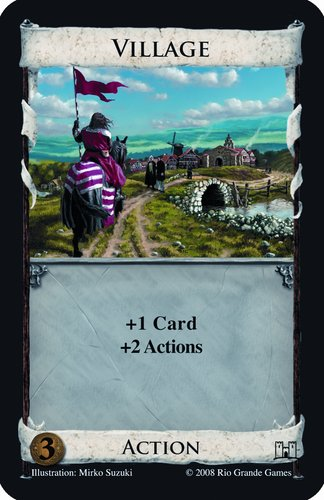
\includegraphics[width=.45\columnwidth]{../pres/village.jpg} \\
    \copyright \cite{dominion}
    \end{flushright}
  \columnbreak
  \begin{flushleft}
    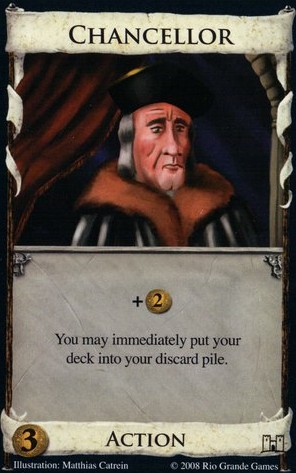
\includegraphics[width=.45\columnwidth]{../pres/chancellor.jpg} \\
    \copyright \cite{dominion}
    \end{flushleft}
\end{multicols}

The two cards above are the \hsk{VILLAGE} and \hsk{CHANCELLOR} cards referred to
throughout this paper. In this case the model parameter $X$ is the \hsk{VILLAGE} and
the model parameter $Y$ is the \hsk{CHANCELLOR}. This is an interesting first pair
of cards to look at because the first buy in a game of Dominion involving these two
cards usually requires the player to choose between buying one of these two cards.
Additionally these cards allow us to make a number of simplifications in the first
iteration of the greedy heuristic. Namely that the optimal play heuristic for a hand
which can only contain these two action cards is to always play \hsk{VILLAGE} cards
first followed by playing any remaining \hsk{CHANCELLOR} cards. This simple action
heuristic is optimal because it maximizes the amount of money the player has during
her subsequent buy phase.

